\documentclass[8pt,a5paper]{article}

\usepackage[english]{babel}
\usepackage[margin=0.6in]{geometry}
\usepackage{siunitx} % Provides the \SI{}{} and \si{} command for typesetting SI units
\usepackage{graphicx} % Required for the inclusion of images
\usepackage{natbib} % Required to change bibliography style to APA
\usepackage{amsmath} % Required for some math elements
\usepackage{longtable}
\usepackage{ragged2e}

\renewcommand{\familydefault}{\sfdefault}
\setlength\parindent{0pt} % Removes all indentation from paragraphs

\newcolumntype{P}[1]{>{\centering\arraybackslash}p{#1}}
\newcolumntype{M}[1]{>{\centering\arraybackslash}m{#1}}
\newcommand{\nomunit}[1]{%
\renewcommand{\nomentryend}{\hspace*{\fill}#1}}

\begin{document}

\pagenumbering{arabic}

\centering
\small

\section*{Small Nuclear Rocket Engine (SNRE) Geometry and Material Configuration}

\raggedright

\subsection*{SNRE Overview}

\begin{table}[h!]
    \label{table: Table 1}
    \centering
    \small
    \caption{Core Overview of the SNRE.}
    \begin{tabular}{|l|l|}
    \hline
    \multicolumn{2}{|l|}{\textbf{Core Overview}}\\\hline
    Uranium Enrichment & $93.0\%$\\
    Total Number of Fuel Elements & $564$\\
    Total Number of Support Elements & $241$\\
    Mass of U235 & \SI{59.6}{kg}\\\hline
    \end{tabular}
\end{table}

\subsection*{Geometry Data}

\begin{table}[h!]
    \label{table: Table 2}
    \centering
    \small
    \caption{Geometry Data of the SNRE Fuel Element}
    \begin{tabular}{|l|l|}
    \hline
    \multicolumn{2}{|l|}{\textbf{Fuel Element Dimensions}}\\\hline
    Flat-to-flat width & \SI{1.905}{cm}\\
    Number of Coolant Channels & $19$\\
    Borehole Diameter & \SI{0.25654}{cm}\\
    Borehole Pitch & \SI{0.40894}{cm}\\
    Internal Coating Thickness & \SI{100}{\mu m}\\
    External Coating Thickness & \SI{50}{\mu m}\\\hline
    \end{tabular}
\end{table}

\begin{table}[h!]
    \label{table: Table 3}
    \centering
    \small
    \caption{Geometry Data of the SNRE Support Element}
    \begin{tabular}{|l|l|}
    \hline
    \multicolumn{2}{|l|}{\textbf{Support Element Dimensions}}\\\hline
    Flat-to-flat width & \SI{1.89484}{cm}\\
    Central Coolant Channel Radius & \SI{0.20955}{cm}\\
    Inner Tie Tube Radius & \SI{0.26035}{cm}\\
    Inner Gap (Stagnant Hydrogen) Radius & \SI{0.26670}{cm}\\
    Moderator Radius & \SI{0.58420}{cm}\\
    Outer Coolant Channel Radius & \SI{0.67818}{cm}\\
    Outer Tie Tube Radius & \SI{0.69850}{cm}\\
    Mid Gap (Stagnant Hydrogen) Radius & \SI{0.70485}{cm}\\
    Insulator Radius & \SI{0.80645}{cm}\\
    Outer Gap (Stagnant Hydrogen) Radius & \SI{0.81280}{cm}\\
    External Coating Thickness & \SI{50.8}{\mu m}\\\hline
    \end{tabular}
\end{table}

\justifying

The external core regions consist of a steel wrapper, beryllium barrel, beryllium
reflector, containing 12 control drums. Positioned above the core is the control
drum actuator zone, brim shield, core support plate, tie tube plenum, and shield
regions. The control drums consist of a cylinder of reflective material, and
control plate of absorptive material, which covers a 120 degree segment of the control drum.

\raggedright

\begin{table}[h!]
    \label{table: Table 4}
    \centering
    \small
    \caption{Geometry Data of the SNRE Core Exterior}
    \begin{tabular}{|m{0.2\linewidth}|m{0.15\linewidth}|m{0.15\linewidth}|m{0.15\linewidth}|m{0.15\linewidth}|}
    \hline
    Region & Inner Radius & Outer Radius& Aft Boundary& Fwd Boundary\\\hline
    Core & - & \SI{29.5275}{cm} & \SI{0.0}{cm} & \SI{89.0}{cm} \\
    Gap & \SI{29.5275}{cm} & \SI{29.8450}{cm} &  \SI{0.0}{cm} & \SI{89.0}{cm} \\
    Stainless-Steel Wrapper & \SI{29.8450}{cm} & \SI{30.1625}{cm} &  \SI{0.0}{cm} & \SI{89.0}{cm} \\
    Gap & \SI{30.1625}{cm} & \SI{30.4800}{cm} &  \SI{0.0}{cm} & \SI{89.0}{cm} \\
    Beryllium Barrel & \SI{30.4800}{cm} & \SI{33.3375}{cm} &  \SI{0.0}{cm} & \SI{89.0}{cm} \\
    Gap & \SI{33.3375}{cm} & \SI{33.6550}{cm} &  \SI{0.0}{cm} & \SI{89.0}{cm} \\
    Beryllium Reflector & \SI{33.6550}{cm} & \SI{43.3870}{cm} & \SI{0.0}{cm} & \SI{89.1}{cm} \\
    Gap & \SI{43.3870}{cm} & \SI{48.7045}{cm} &  \SI{0.0}{cm} & \SI{129.640}{cm} \\
    Pressure Vessel & \SI{48.7045}{cm} & \SI{49.2633}{cm} &  \SI{0.0}{cm} & \SI{129.640}{cm} \\
    Lower Tie Tube Plenum & - & \SI{33.6550}{cm} & \SI{89.0}{cm} & \SI{96.62}{cm} \\
    Core Support Plate & - & \SI{33.6550}{cm} & \SI{96.62}{cm} & \SI{106.78}{cm} \\
    Upper Tie Tube Plenum & - & \SI{33.6550}{cm} & \SI{106.78}{cm} & \SI{111.86}{cm} \\
    Lower Internal Shield & - & \SI{33.6550}{cm} & \SI{111.86}{cm} & \SI{119.734}{cm} \\
    Hydrogen Plenum & - & \SI{33.6550}{cm} & \SI{119.734}{cm} & \SI{121.766}{cm} \\
    Upper Internal Shield & - & \SI{33.6550}{cm} & \SI{121.766}{cm} & \SI{129.640}{cm} \\
    Control Drum Actuator Zone & \SI{33.6550}{cm} & \SI{43.3870}{cm} & \SI{89.1}{cm} & \SI{111.860}{cm} \\
    Brim Shield & \SI{33.6550}{cm} & \SI{48.3870}{cm} & \SI{111.860}{cm} & \SI{119.734}{cm} \\
    Hydrogen Plenum & \SI{33.6550}{cm} & \SI{48.3870}{cm} & \SI{119.734}{cm} & \SI{129.640}{cm} \\\hline
    \end{tabular}
\end{table}

\begin{table}[h!]
    \label{table: Table 5}
    \centering
    \small
    \caption{Geometry Data of the SNRE Control Drum}
    \begin{tabular}{|l|l|}
    \hline
    \multicolumn{2}{|l|}{\textbf{Control Drum Dimensions}}\\\hline
    Control Drum Radius & \SI{6.0325}{cm}\\
    Control Plate Inner Radius & \SI{5.3975}{cm}\\
    Control Plate Thickness & \SI{0.635}{cm}\\\hline
    \end{tabular}
\end{table}

\subsection*{Material Data}

\begin{longtable}{|m{0.2\linewidth}|m{0.25\linewidth}|m{0.25\linewidth}|}
    \caption{Material Data of the SNRE Support Element} \\
    
    \hline \textbf{Material} & \textbf{Atom Density $(\SI{}{atoms/bn \cdot cm3})$} & \textbf{Mass Density $(\SI{}{g/cm3})$ and} w/o \\ \hline 
    \endfirsthead
    
    
    \hline \textbf{Material} & \textbf{Atom Density $(\SI{}{atoms/bn \cdot cm3})$} & \textbf{Mass Density $(\SI{}{g/cm3})$ and} w/o \\ \hline 
    \endhead
    
    \hline \multicolumn{3}{|r|}{{Continued on next page}} \\ \hline
    \endfoot
    
    \hline
    \endlastfoot
    \multicolumn{3}{|c|}{\textbf{Fuel Element Coolant}}\\\hline
    Density & - & - \\
    H & \SI{1.61317E-03}{}& - \\\hline
    \multicolumn{3}{|c|}{\textbf{Fuel}}\\\hline
    Density & - & \SI{3.64}{} \\
    U & - & \SI{0.60}{} \\
    Zr & - & \SI{1.81}{} \\
    C & - & \SI{1.23}{} \\\hline
    \multicolumn{3}{|c|}{\textbf{Fuel Coating}}\\\hline
    Density (100\%) & - & \SI{6.73}{} \\
    C & - & \SI{0.11625}{} \\
    Zr & - & \SI{0.88375}{} \\
\end{longtable}

\begin{longtable}{|m{0.2\linewidth}|m{0.25\linewidth}|m{0.25\linewidth}|}
    \caption{Material Data of the SNRE Support Element} \\
    
    \hline \textbf{Material} & \textbf{Atom Density $(\SI{}{atoms/bn \cdot cm3})$} & \textbf{Mass Density $(\SI{}{g/cm3})$ and} w/o \\ \hline 
    \endfirsthead
    
    
    \hline \textbf{Material} & \textbf{Atom Density $(\SI{}{atoms/bn \cdot cm3})$} & \textbf{Mass Density $(\SI{}{g/cm3})$ and} w/o \\ \hline 
    \endhead
    
    \hline \multicolumn{3}{|r|}{{Continued on next page}} \\ \hline
    \endfoot
    
    \hline
    \endlastfoot
    \multicolumn{3}{|c|}{\textbf{Support Element Coolant}}\\\hline
    Density & - & - \\
    H & \SI{1.61317E-03}{}& - \\\hline
    \multicolumn{3}{|c|}{\textbf{Stagnant Hydrogen}}\\\hline
    Density & - & - \\
    H & \SI{1.9127E-03}{}& - \\\hline
    \multicolumn{3}{|c|}{\textbf{Inconel 718}}\\\hline
    Density & - & \SI{8.19}{} \\
    B & \SI{0.000023}{} & \SI{0.000050}{} \\
    C & \SI{0.000300}{} & \SI{0.000730}{} \\
    Al & \SI{0.000914}{} & \SI{0.005000}{} \\
    Si & \SI{0.000558}{} & \SI{0.003180}{} \\
    P & \SI{0.000022}{} & \SI{0.000140}{} \\
    S & \SI{0.000022}{} & \SI{0.000140}{} \\
    Ti & \SI{0.000927}{} & \SI{0.009000}{} \\
    Cr & \SI{0.018023}{} & \SI{0.190000}{} \\
    Mn & \SI{0.000285}{} & \SI{0.003180}{} \\
    Fe & \SI{0.015014}{} & \SI{0.170000}{} \\
    Ni & \SI{0.044117}{} & \SI{0.525000}{} \\
    Co & \SI{0.000762}{} & \SI{0.009100}{} \\
    Cu & \SI{0.000212}{} & \SI{0.002730}{} \\
    Nb & \SI{0.002721}{} & \SI{0.051250}{} \\
    Mo & \SI{0.001568}{} & \SI{0.030500}{} \\\hline
    \multicolumn{3}{|c|}{\textbf{Moderator}}\\\hline
    Density & - & \SI{5.61}{} \\
    C & - & \SI{0.017582}{} \\
    Zr & - & \SI{0.98241}{} \\\hline
    \multicolumn{3}{|c|}{\textbf{Insulator}}\\\hline
    Density (50\%) & - & \SI{3.365}{} \\
    C & - & \SI{0.11625}{} \\
    Zr & - & \SI{0.88375}{} \\\hline
    \multicolumn{3}{|c|}{\textbf{Support Element Sleeve}}\\\hline
    Density & - & \SI{1.70}{} \\
    C & \SI{0.085238}{} & \SI{0.999999}{} \\
    B & \SI{0.000000}{} & \SI{0.000001}{} \\\hline
    \multicolumn{3}{|c|}{\textbf{Support Element Coating}}\\\hline
    Density (100\%) & - & \SI{6.73}{} \\
    C & - & \SI{0.11625}{} \\
    Zr & - & \SI{0.88375}{} \\
\end{longtable}

Note that the insulator region is porous ZrC at 50\% porosity. The support
element contains regions of stagnant hydrogen.

\begin{longtable}{|m{0.2\linewidth}|m{0.25\linewidth}|m{0.25\linewidth}|}
    \caption{Material Data of the SNRE Core Exterior} \\
    
    \hline \textbf{Material} & \textbf{Atom Density $(\SI{}{atoms/bn \cdot cm3})$} & \textbf{Mass Density $(\SI{}{g/cm3})$ and} w/o \\ \hline 
    \endfirsthead
    
    
    \hline \textbf{Material} & \textbf{Atom Density $(\SI{}{atoms/bn \cdot cm3})$} & \textbf{Mass Density $(\SI{}{g/cm3})$ and} w/o \\ \hline 
    \endhead
    
    \hline \multicolumn{3}{|r|}{{Continued on next page}} \\ \hline
    \endfoot
    
    \hline
    \endlastfoot
    \multicolumn{3}{|c|}{\textbf{Steel Wrapper (SS-347)}}\\\hline
    Density & - & \SI{8.19}{} \\
    C & \SI{0.000023}{} & \SI{0.000050}{} \\
    Si & \SI{0.000300}{} & \SI{0.000730}{} \\
    P & \SI{0.000914}{} & \SI{0.005000}{} \\
    S & \SI{0.000558}{} & \SI{0.003180}{} \\
    Cr & \SI{0.000022}{} & \SI{0.000140}{} \\
    Mn & \SI{0.000022}{} & \SI{0.000140}{} \\
    Fe & \SI{0.000927}{} & \SI{0.009000}{} \\
    Ni & \SI{0.018023}{} & \SI{0.190000}{} \\
    Nb & \SI{0.000285}{} & \SI{0.003180}{} \\
    Ta & \SI{0.015014}{} & \SI{0.170000}{} \\\hline
    \multicolumn{3}{|c|}{\textbf{Beryllium Barrel}}\\\hline
    Density & - & - \\
    Be & \SI{1.9127E-03}{}& - \\\hline
    \multicolumn{3}{|c|}{\textbf{Reflector}}\\\hline
    Density & - & \SI{8.19}{} \\
    Be & \SI{0.000023}{} & \SI{0.000050}{} \\\hline
    \multicolumn{3}{|c|}{\textbf{Control Drum}}\\\hline
    Density & - & \SI{5.61}{} \\
    Be & - & \SI{0.98241}{} \\\hline
    \multicolumn{3}{|c|}{\textbf{Control Plate}}\\\hline
    Density (50\%) & - & \SI{3.365}{} \\
    Hf & - & \SI{0.88375}{} \\\hline
    \multicolumn{3}{|c|}{\textbf{Lower Tie Tube Plenum}}\\\hline
    Density & - & \SI{1.70}{} \\
    H & \SI{0.085238}{} & \SI{0.999999}{} \\
    Fe & \SI{0.000000}{} & \SI{0.000001}{} \\\hline
    \multicolumn{3}{|c|}{\textbf{Core Support Plate}}\\\hline
    Density (100\%) & - & \SI{6.73}{} \\
    H & \SI{0.085238}{} & \SI{0.999999}{} \\
    Fe & \SI{0.000000}{} & \SI{0.000001}{} \\\hline
    \multicolumn{3}{|c|}{\textbf{Upper Tie Tube Plenum}}\\\hline
    Density & - & \SI{1.70}{} \\
    H & \SI{0.085238}{} & \SI{0.999999}{} \\
    Fe & \SI{0.000000}{} & \SI{0.000001}{} \\\hline
    \multicolumn{3}{|c|}{\textbf{Lower Internal Shield}}\\\hline
    Density (100\%) & - & \SI{6.73}{} \\
    H & - & \SI{0.11625}{} \\
    B & \SI{0.085238}{} & \SI{0.999999}{} \\
    Zr & \SI{0.000000}{} & \SI{0.000001}{} \\\hline
    \multicolumn{3}{|c|}{\textbf{Hydrogen Plenum}}\\\hline
    Density & - & \SI{1.70}{} \\
    H & \SI{0.000000}{} & \SI{0.000001}{} \\\hline
    \multicolumn{3}{|c|}{\textbf{Upper Internal Shield}}\\\hline
    Density (100\%) & - & \SI{6.73}{} \\
    H & - & \SI{0.11625}{} \\
    B & \SI{0.085238}{} & \SI{0.999999}{} \\
    Zr & \SI{0.000000}{} & \SI{0.000001}{} \\\hline
    \multicolumn{3}{|c|}{\textbf{Control Drum Actuator Zone}}\\\hline
    Density & - & \SI{1.70}{} \\
    H & - & \SI{0.11625}{} \\
    Fe & \SI{0.085238}{} & \SI{0.999999}{} \\
    Cu & \SI{0.000000}{} & \SI{0.000001}{} \\\hline
    \multicolumn{3}{|c|}{\textbf{Brim Shield}}\\\hline
    Density (100\%) & - & \SI{6.73}{} \\
    H & - & \SI{0.11625}{} \\
    B & \SI{0.085238}{} & \SI{0.999999}{} \\
    Zr & \SI{0.000000}{} & \SI{0.000001}{} \\\hline
    \multicolumn{3}{|c|}{\textbf{Pressure Vessel}}\\\hline
    Density & - & \SI{1.70}{} \\
    Al & \SI{0.000000}{} & \SI{0.000001}{} \\
\end{longtable}

\begin{figure}[h!]
    \centering
    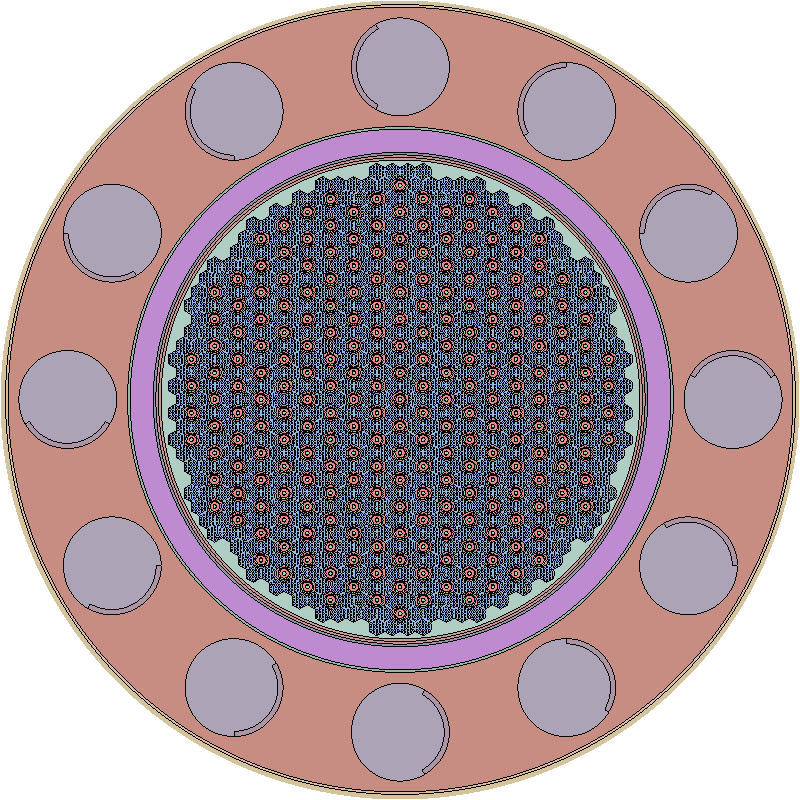
\includegraphics[width=1\linewidth]{figures/Reactor.png}
    \caption{Model of the Core with Drums at the Critical Position (90 degrees)}
    \label{fig:Figure 1}
\end{figure}

\end{document}
